\section{Current investigations}

\begin{frame}{How to check Gianluca's remaining bottleneck}{}
	\begin{center} 
		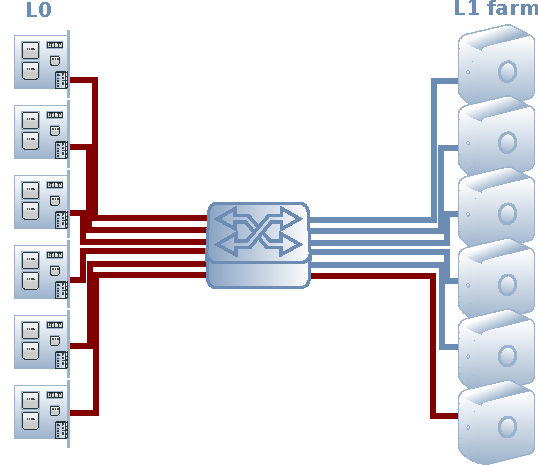
\includegraphics[height=7cm]{gianlucas-bottleneck}
	\end{center} 
\end{frame}

\begin{frame}{How to check Gianluca's remaining bottleneck}{Check latencies}
	\begin{block}{First idea: measure relative latency}
		\begin{itemize}
		  \item Let X PCs send N frames containing the sending time
		  \item Calculate difference between timestamp in received package and the
		  time of reception 
		  \item Forget about the accuracy as you cannot synch the clocks, but\ldots
		  \item This value should increase rapidly if you have problems with too big X
		  and N
		\end{itemize}
	\end{block}
	\begin{alertblock}{Large drift}
		Even miliseconds after an NTP-synchronization with a stratum 3 the drift
		between L0 clocks and L1 clock is much too large (about 50µs per second)
	\end{alertblock}
\end{frame}

\begin{frame}{How to check Gianluca's remaining bottleneck}{Check data rate and
packet loss}
	\begin{block}{Better idea: measure the packet loss}
		I used 21 simulated L0-Machines (on 12 PCs, 21*1G links) and one big
		L1-Machine (one 10G link) on on HP PC6248 switch for following procedure:
	\end{block}
	
	\begin{itemize}
	  \item L0TP sends broadcast (frame size X and number of frames N)
	  \item L0-Machines send N frames of size X to one L1 PC
	  \item Now we have a bundle of 21*N frames going to L1
	  \item L1 counts the frames $\rightarrow$ calculates packet loss and data rate
	  \item L1 can separate the bundles by numbers in the frames (frames are not
	  ordered!)
	\end{itemize}
\end{frame}

\begin{frame}{What I will show}{}
	I will only show results with a data rate higher than 300MBps.  
\end{frame}

\begin{frame}{Bundle rate}{}
	\begin{center} 
		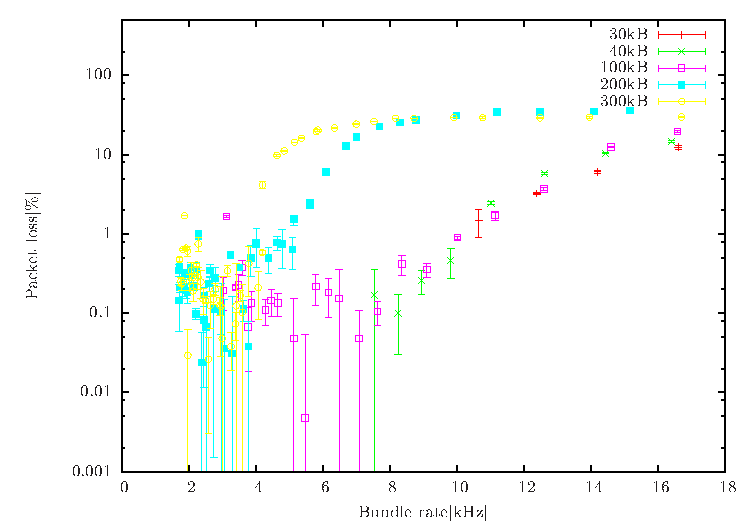
\includegraphics[height=7cm]{rate}
	\end{center} 
\end{frame}

\begin{frame}{Bundle size}{}
	\begin{center} 
		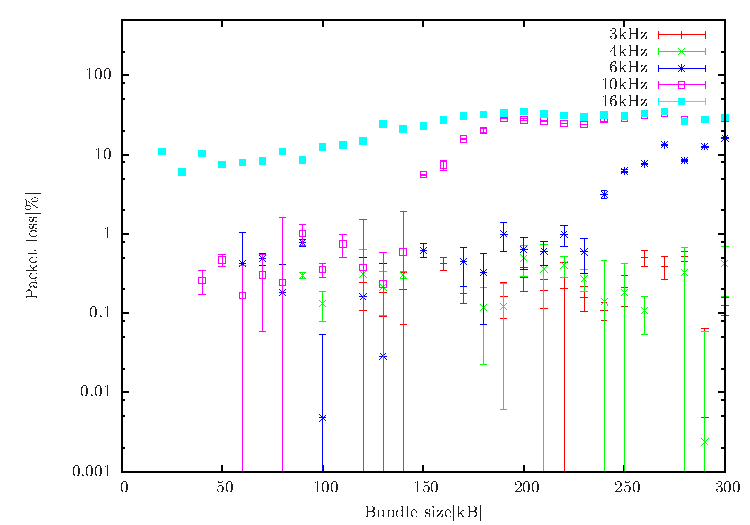
\includegraphics[height=7cm]{data}
	\end{center} 
\end{frame}

\begin{frame}{Overview heat map}{All rates}
	\begin{center} 
		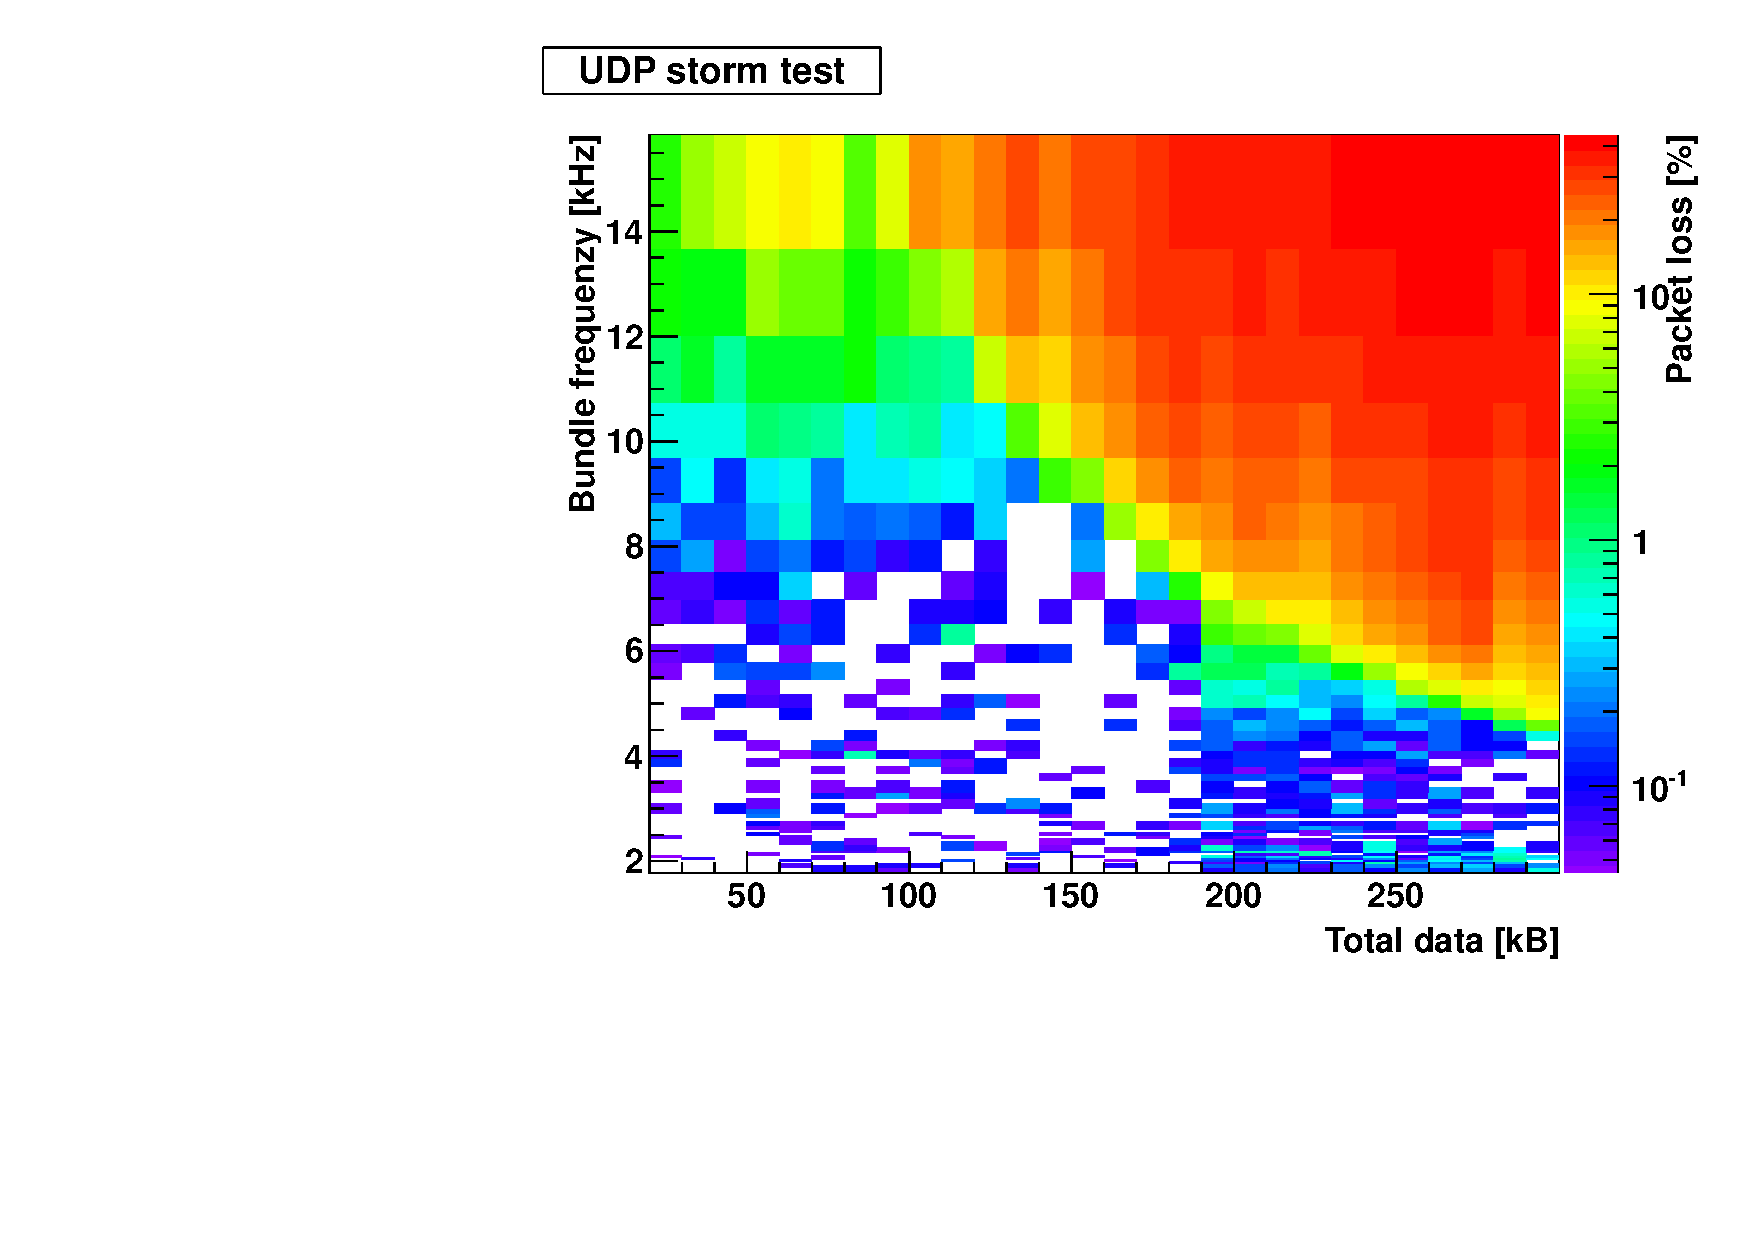
\includegraphics[height=7cm]{heat}
	\end{center} 
\end{frame}

\begin{frame}{Overview heat map}{Only 10Gbps}
	\begin{center} 
		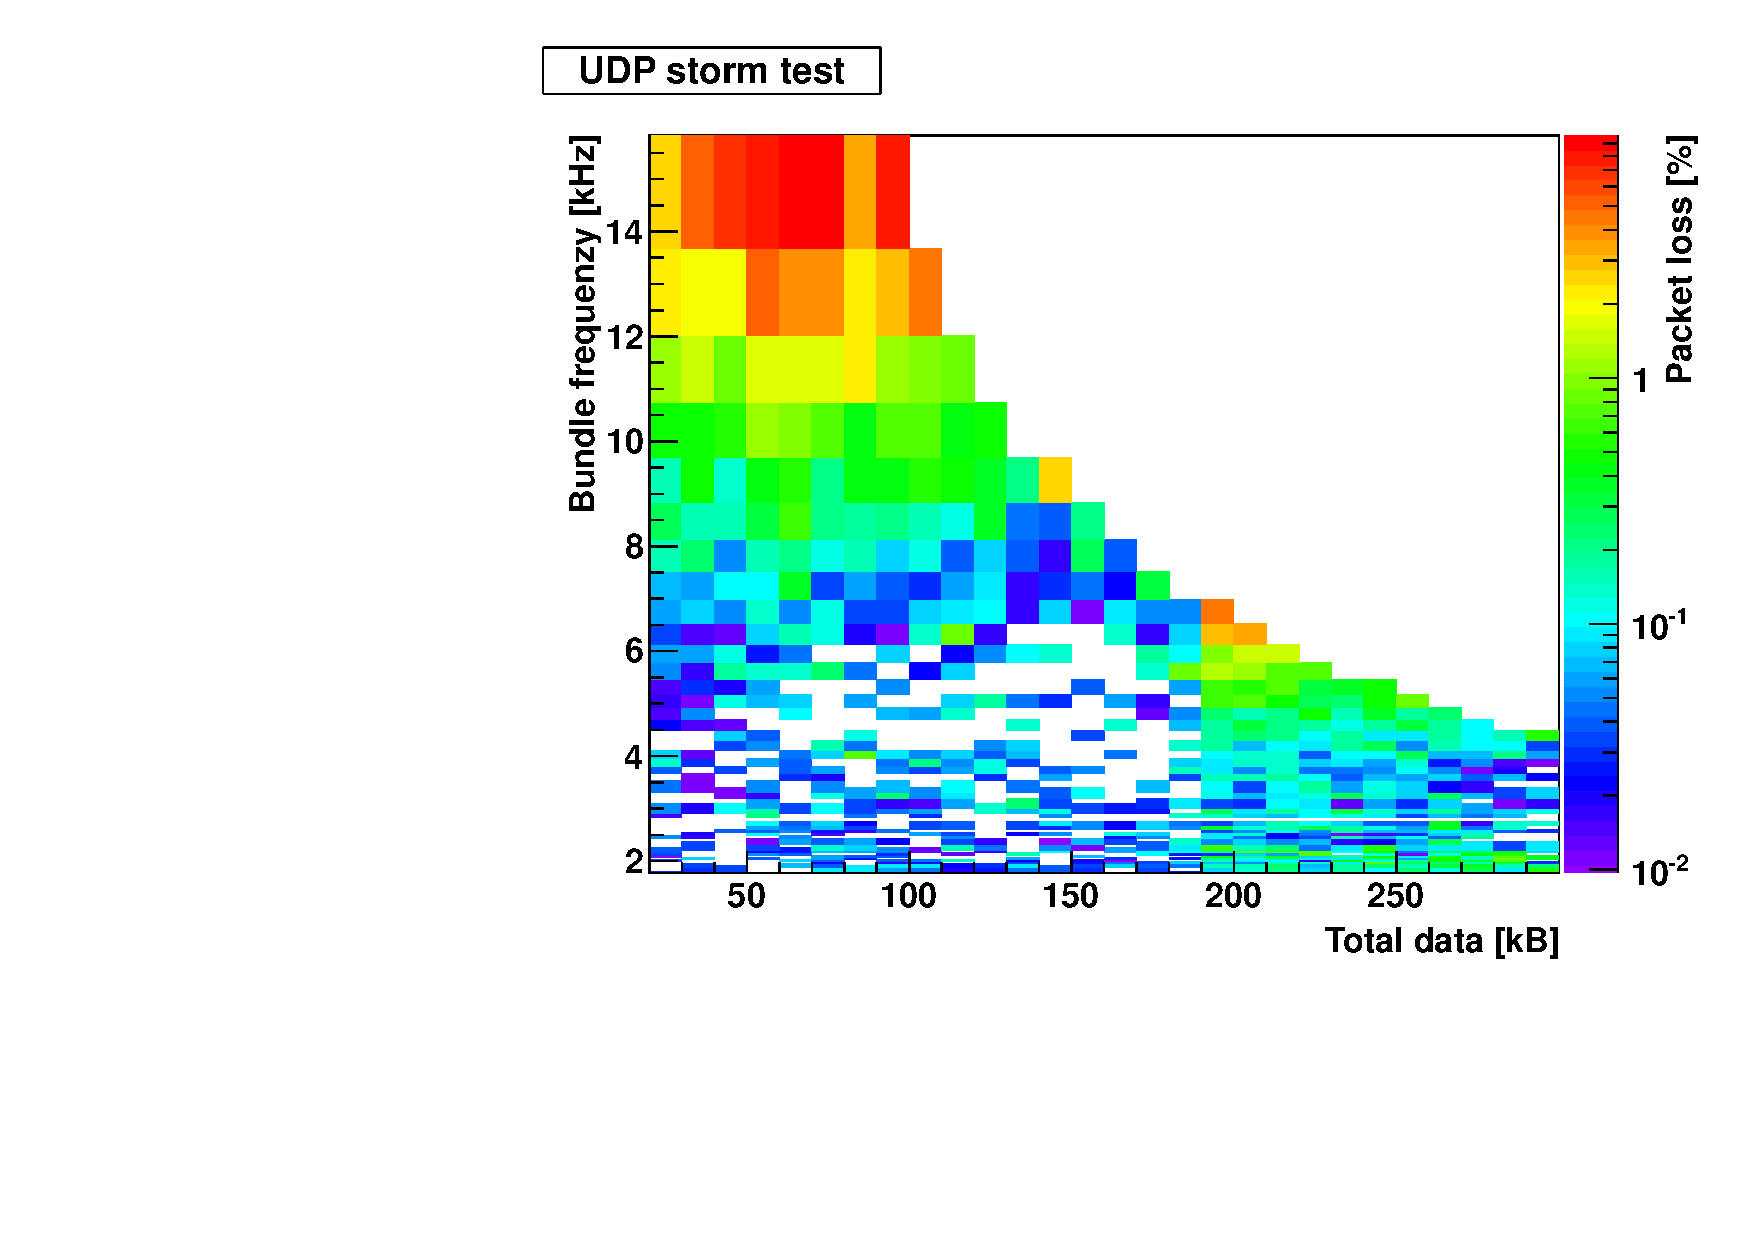
\includegraphics[height=7cm]{heat-10G}
	\end{center} 
\end{frame}

\begin{frame}{Overview heat map}{Bundle frequency vs sleeping time at L0}
	\begin{center} 
		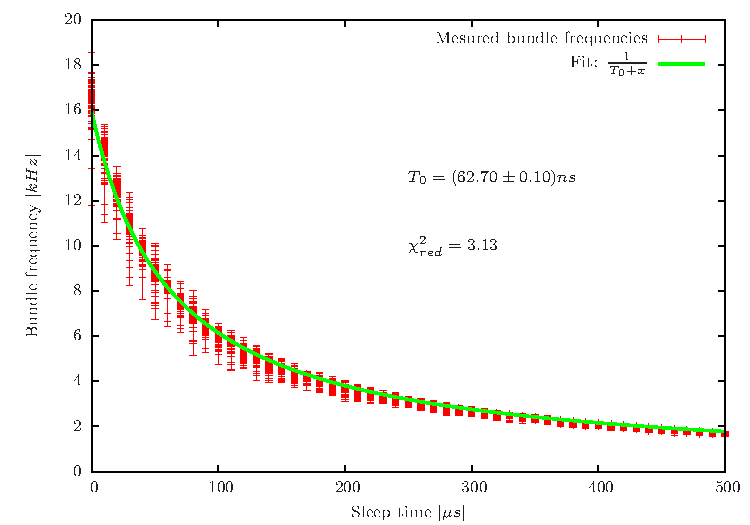
\includegraphics[height=7cm]{frequency}
	\end{center} 
\end{frame}

\begin{frame}{HP: Distributed trunking}{}
	\begin{center} 
		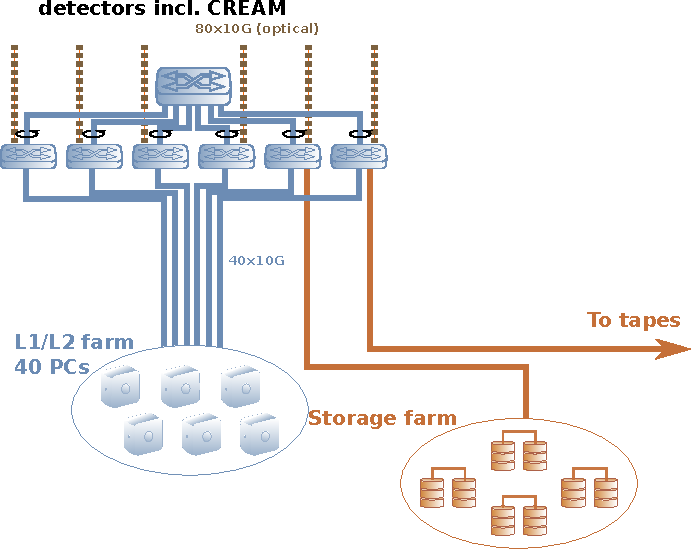
\includegraphics[height=7cm]{whole-farm-l12merged-tree}
	\end{center} 
\end{frame}

\begin{frame}{Hexapus topology}{}
	\begin{center} 
		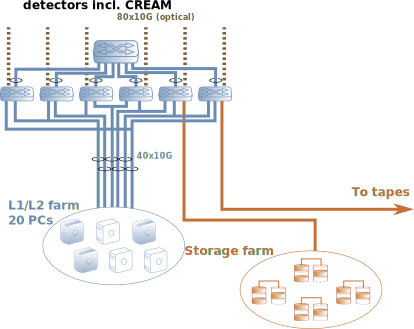
\includegraphics[height=7cm]{farm-merged-hexapus-distributed-trunks}
	\end{center} 
\end{frame}